\documentclass[a4paper,10pt]{article}

\usepackage{graphicx}
\usepackage[utf8]{inputenc}
\usepackage[spanish]{babel}
\usepackage[left=2cm,top=3cm,right=2cm]{geometry}
\usepackage{lgrind}

\title{\PWB \\ Framework Multipropósito de Aplicaciones Web sobre PHP}

\date{}
\author{
\begin{tabular}[t]
{c@{\extracolsep{5em}}c}
Alejandro Siri & Mariano Montone \\
Eureka Consulting & Eureka Consulting \\
Calle 11 Nro 684 & Calle 11 Nro 684 \\
La Plata, 1900, Argentina & La Plata, 1900, Argentina \\
+54 221 489 5591 & +54 221 489 5591 \\
asiri@eureka-consulting.com.ar & mmontone@eureka-consulting.com.ar
\end{tabular}
}

\newcommand{\comment}[1]{}
\newcommand{\PITS}{\emph{Programming in the Small}} %en.wikipedia.org/wiki/Programming_in_the_small
\newcommand{\PWB}{\emph{PHPWebBuilder}}

\newcommand{\sourcecode}[1]{
#1
}

\begin{document}

\maketitle

\abstract{
%El enfoque puede ser puramente tecnico, comentando los como, por que, quienes, cuanto y cuando hicieron el proyecto. Desde la elección de herramientas, problemas tecnicos encontrados, etc. o lo que consideren.
%
%También, si lo tiene, se puede incluir algun condimento respecto de que utilidad/visión (social/empresarial/politica) aporta el proyecto.
El diseño y desarrollo de aplicaciones (tanto de escritorio como web) plantea muchos problemas reiterativos. Existen múltiples soluciones para cada una de ellas, cargando sobre el programador la responsabilidad de seleccionarlas e integrarlas. \PWB\ es un Framework Open Source Orientado a Objetos escrito en PHP para el desarrollo de aplicaciones Web, tanto de Internet como de una Intranet, que integra soluciones a cada uno de estos problemas, elegidas en base a nuestra experiencia en el desarrollo de este tipo de aplicaciones.

{\bf Keywords}: Templates declarativos, desarrollo por componentes, mapeo objeto-relacional bajo persistencia por alcance, distintos engines de rendereo, compilación y macros.

}

% \section{Nombre}
% En un principio, Perseus fue llamado PHPWebBuilder (porque era utilizado para hacer webs en PHP). Luego de muchas modificaciones al framework, decidimos
% rebautilzarlo. El nombre Perseus fue elegido por la mitología griega, ya que este era un heroe que, con ayuda de muchas herramientas, pudo acabar
% al monstruo Medusa, que convertía a sus contrincantes en piedra.
%
% En un principio, Perseus fue llamado PHPWebBuilder (porque era utilizado para hacer webs en PHP). Luego de muchas modificaciones al framework decidimos rebautilzarlo. El nombre Perseus fue elegido por la mitología griega, ya que este era un heroe que, con ayuda de muchas herramientas, pudo acabar al monstruo Medusa, que convertía a sus contrincantes en piedra.
%
% Perseus, gracias a la integración de sus múltiples herramientas, sirve para atacar desde proyectos pequeños hasta los más grandes, que petrifican hasta a los mejores programadores.
%
% \section{Origenes}
%
% En un principio, Perseus fue diseñado para desarrollo de sitios web. Las ventajas principales las presentaba en cuanto a lo que es persistencia y mapeo Objeto-Relacional bajo PHP, además de contar con un CMS con permisos de acceso.
%
% Luego, se le implementó el framework de componentes, templates y de eventos, con lo que se pudo empezar con los primeros sistemas de intranet.
%
% En las últimas versiones, con el manejo de macros, oql, y compilación, los proyectos se simplifican cada vez más.
%
% \section{Tecnologías de soporte}
%
% La elección inicial de LAMP, para aplicaciones web, era evidente, por el amplio alcance de estas tecnologías en los servidores comerciales web.
%
% Ante la mayor cantidad de opciones para hacer software de escritorio e intranet, nos vimos inclinados por las tecnologías web, por la facilidad de distribución y la escalabilidad de la misma.
%
% Al haber elegido LAMP nos vimos forzados a desarrollar en PHP. Si bien tiene limitaciones, PHP resultó tener buen soporte, además de ser un lenguaje flexible, lo que permite hacer diseños fácilmente modificables.
%
% }

\section{Introducción}

El diseño y desarrollo de aplicaciones (tanto de escritorio como web) plantea muchos problemas reiterativos. La interacción con el usuario, la presentacion de la información y el almacenamiento y recuperación de la misma son algunos de los más frecuentes y que más tiempo consumen.
Por esto mismo son foco de mucha invesigación y trabajo, habiendo conseguido a lo largo de los años múltiples soluciones. Seleccionar e integrar éstas queda a cargo del programador o grupo de trabajo de un proyecto específico.

\PWB \ es un framework de desarrollo que integra múltiples soluciones que en nuestra experiencia mejoran el tiempo de desarrollo y la calidad del producto de software sin sacrificar flexibilidad en el diseño.

%\section{\PWB}

El framework está diseñado bajo una arquitectura MVC (Model-view-controller)\cite{mvc}.
Esto quiere decir que una aplicación se compone de 3 capas:
\begin{itemize}
\item El \emph{Modelo}. Es la representación de la información de dominio específico de la aplicación.
\item El \emph{Controlador}. Está basada en la programación de componentes. Responden a la acción del usuario y definen los aspectos navigacionales de la aplicación (más sobre ésto en la sección \ref{sec-controller}).
\item La \emph{Vista}. La forma en la que se presentan los datos y botones que el usuario ve se define a través de templates declarativos, HTML y CSS. Desarrollamos los aspectos de presentación en la sección \ref{sec-view}.
\end{itemize}

Existe una parte más que integra el framework. Esto es la ``Programación en lo pequeño'' (\PITS), la programación de los módulos y funciones del programa, que sirven para unir estas capas. Los frameworks actuales ayudan a simplificar el desarrollo bajo MVC; el soporte para la \PITS \ generalmente es dependiente del lenguaje/plataforma. \PWB \ se apoya en PHP para parte de esta tarea, y además provee al desarrollador herramientas para solucionar o simplificar las tareas en las otras areas:

\begin{itemize}
\item Para el modelo, presenta un mapeo automático de base de datos (sección \ref{sub-pers}), autogeneración del esquema de base de datos (sección \ref{sub-adapt}), y un lenguaje de consultas complejas (sección \ref{sub-oql}) que tiene en cuenta la herencia del modelo de clases.  Esto permite que la tarea del desarrollador se limite a enfocarse a resolver la problemática que plantea el diseño del modelo.

\item Para el controlador, utiliza un sistema de componentes (sección \ref{sub-comp}), que permiten reusar ``pedazos de aplicación'' , ya sea en diferentes partes de una misma aplicación o en diferentes proyectos. Además, los widgets (sección \ref{sub-widget}) simplifican y encapsulan la interacción con el usuario.

\item Para la vista, el sistema de templates (sección \ref{sub-templates}) basados en XML permiten una adaptación directa del trabajo de un diseñador gráfico (sección \ref{sub-templates-adapt}). El sistema se encarga de presentar la información utilizando AJAX de manera transparente, u otra forma de rendereo (sección \ref{sub-render}) (esto es fácilmente configurable).

\item Por último, para \PITS, \PWB \ presenta una serie de características disponibles en otros lenguajes y plataformas pero no existentes en PHP. Estas son una implementación de Eventos (sección \ref{sub-events}),
%Weak References (sección \ref{sub-weak}),
%creación de DSLs (sección \ref{sub-phpcc}),
%Mixins (sección \ref{sub-mixins}).
y Macros (sección \ref{sub-macros}).

\end{itemize}

\section{Características del Modelo}

Para ejemplificar, veremos la creación de un blog (figura \ref{fig-blog1}).

\begin{figure}[h]
	\centering
	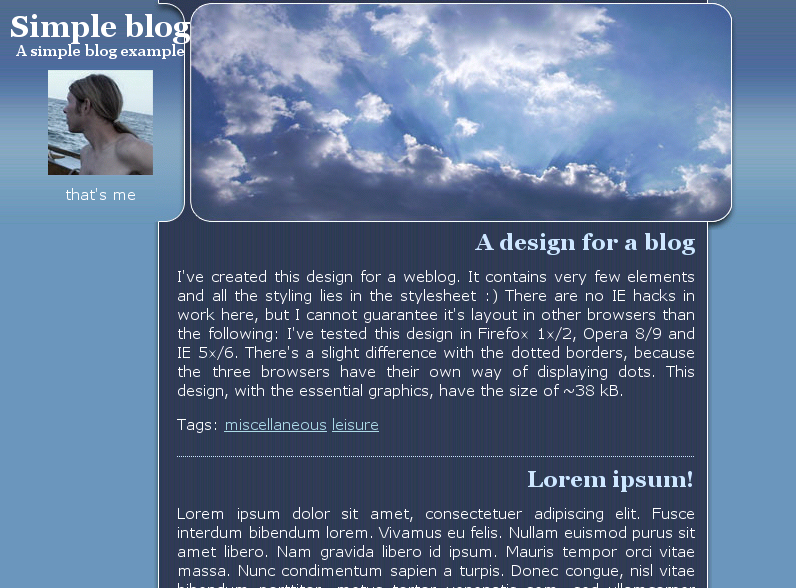
\includegraphics[scale=0.6]{images/blog1.png}
 	\caption{Nuestro blog}
 	\label{fig-blog1}
\end{figure}

Las tareas a realizar son:
\begin{enumerate}
\item Crear el modelo de clases.
\item Decidir cuáles son las formas de interacción de los usuarios con el sistema.
\item Presentar esas formas de interacción de una manera atractiva y entendible para el usuario.
\end{enumerate}

\subsection{Diseño de la aplicación}

El Modelo de la aplicación, es la representación de la información de dominio específico de la aplicación. Para el blog, tendremos las siguientes clases: \emph{Post}, \emph{Tag}, \emph{User} (figura \ref{fig-model1}).

\begin{figure}[ht]
	\centering
	\includegraphics*[scale=0.50,viewport=420 350 700 600]{images/diagrama.png}
 	\caption{Modelo de objetos del Blog}
 	\label{fig-model1}
\end{figure}


\subsection{Persistencia y metadata}
\label{sub-pers}

Los datos del modelo necesitan en general ser persistidos para que éstos puedan ser accedidos en otra ejecución de la aplicación, ya sea simultánea o posterior.

\PWB \ posee un mecanismo para la persistencia que permite, mediante anotaciones especiales en los datos del modelo, el guardado y recuperación automática de los datos en la base de datos.

La persistencia del modelo se consigue mediante la subclasificación de la clase especial \verb"PersistentObject". Esta clase provee la funcionalidad necesaria para describir la metadata en su inicialización y también para las operaciones de guardado y borrado.

De esta manera declaramos la clase \verb"Post":

\sourcecode{src/Post.class.php.tex}

Esto define una clase persistente \verb"Post". En ella definimos un método initialize en el que declaramos los atributos que tiene un \verb"Post". En este caso son un \emph{título} (\verb"title"), un \emph{texto} (\verb"text"), una colección de \emph{etiquetas} (\verb"tags") y el usuario \emph{autor} (\verb"author"). La definición de un atributo se hace invocando el método \verb"addField" de \verb"PersistentObject" con el tipo de campo que queremos crear.

La clase \verb'PersistentObject' posee los métodos \verb'save' y \verb'delete', que permiten insertar, actualizar y borrar objetos de la base de datos.

Para crear y guardar un \verb'Post' de título 'Model persistence' hacemos:

\sourcecode{src/CreatePost.php.tex}

Esto deja el \verb'Post' persistido en la base de datos.

\subsection{Recuperación de objetos}

Una operación habitual en el desarrollo de una aplicación es la recuperación de datos y de información calculada en base a estos.

La recuperación de objetos en \PWB \ se hace mediante la clase \verb"Report" que permite obtener los objetos de una colección, filtrada por varios criterios y ordenada. Estos reportes tienen en cuenta las subclases de los objetos y utilizan herencia para las variables de instancia.

Para obtener todos los \verb"Posts" cuya etiqueta sea una dada creamos el siguiente objeto Report:

\sourcecode{src/ReportTest.php.tex}

Esta consulta, genera el siguiente SQL:

\sourcecode{src/consulta.sql.tex}

Como podemos ver, no se acorta la cantidad de código escrito pero se simplifica. Alcanza con determinar la clase sobre la que hace la consulta (\verb"Post") e indicar las restricciones (en este caso, que solamente queremos aquellos Post que posean a \verb'$tag' entre los elementos de su colección). %$

El programador no tiene que preocuparse por seleccionar correctamente los campos del objeto. Los joins de tablas se hacen automáticamente (incluso los de herencia, en este ejemplo no se nota por su simplicidad).

La principal ventaja de generar las consultas es que un cambio en las clases del modelo no implica necesariamente modificar las consultas a mano (por ejemplo, si agregásemos un campo `fecha de publicación' en el \verb"Post"). Esto mejora notablemente la productividad.

\subsection{OQL (Object Query Language)}
\label{sub-oql}
Dada la complejidad de construir un reporte completo a mano, desarrollamos un lenguaje \emph{OQL} para consulta de los objetos. Usando esto, para obtener todos los \verb"Posts" cuya etiqueta sea una dada, creamos esta consulta:

\begin{verbatim}
#@select p:Post where exists (p.tags as tag where tag.name=$tag)@#;
\end{verbatim}

Vemos que la complejidad de crear el reporte se disminuye en una alta proporción.
La extraña sintaxis (los tokens \verb"#@" \verb"@#" que encierran la expresión de consulta) corresponde a la utilización de macros, que veremos en la sección \ref{sub-macros}.

Una buena propiedad del lenguaje es que está íntimamente relacionado con el código PHP, ya que puede utilizar las variables en el scope (es decir, el OQL está embebido en el PHP).

Para buscar los post que tengan el tag  \verb"$tag", %$
agregamos en la clase \verb"Post" el siguiente mensaje de clase:

\sourcecode{src/PostwOQL.class.php.tex}

\subsection{Adaptación de base de datos}
\label{sub-adapt}

Para poder persistir los datos del modelo, se necesita un repositorio. \PWB\ utiliza una base de datos relacional para ello y realiza un mapeo Objeto-Relacional de los datos. Para poder realizar este mapeo, es necesario que la base de datos mantenga una estructura específica.

La estructura necesaria para la persistencia del modelo se puede inferir de la definición de los objetos, donde establecemos los tipos de las variables de cada clase y las relaciones de subclasificación.

\PWB \ genera el esquema automáticamente librando al programador de esta carga, que es generalmente hasta más larga (y muchísimo más tediosa) que la programación del modelo (figura \ref{fig-admin1}).

\begin{figure}[h]
	\centering
	%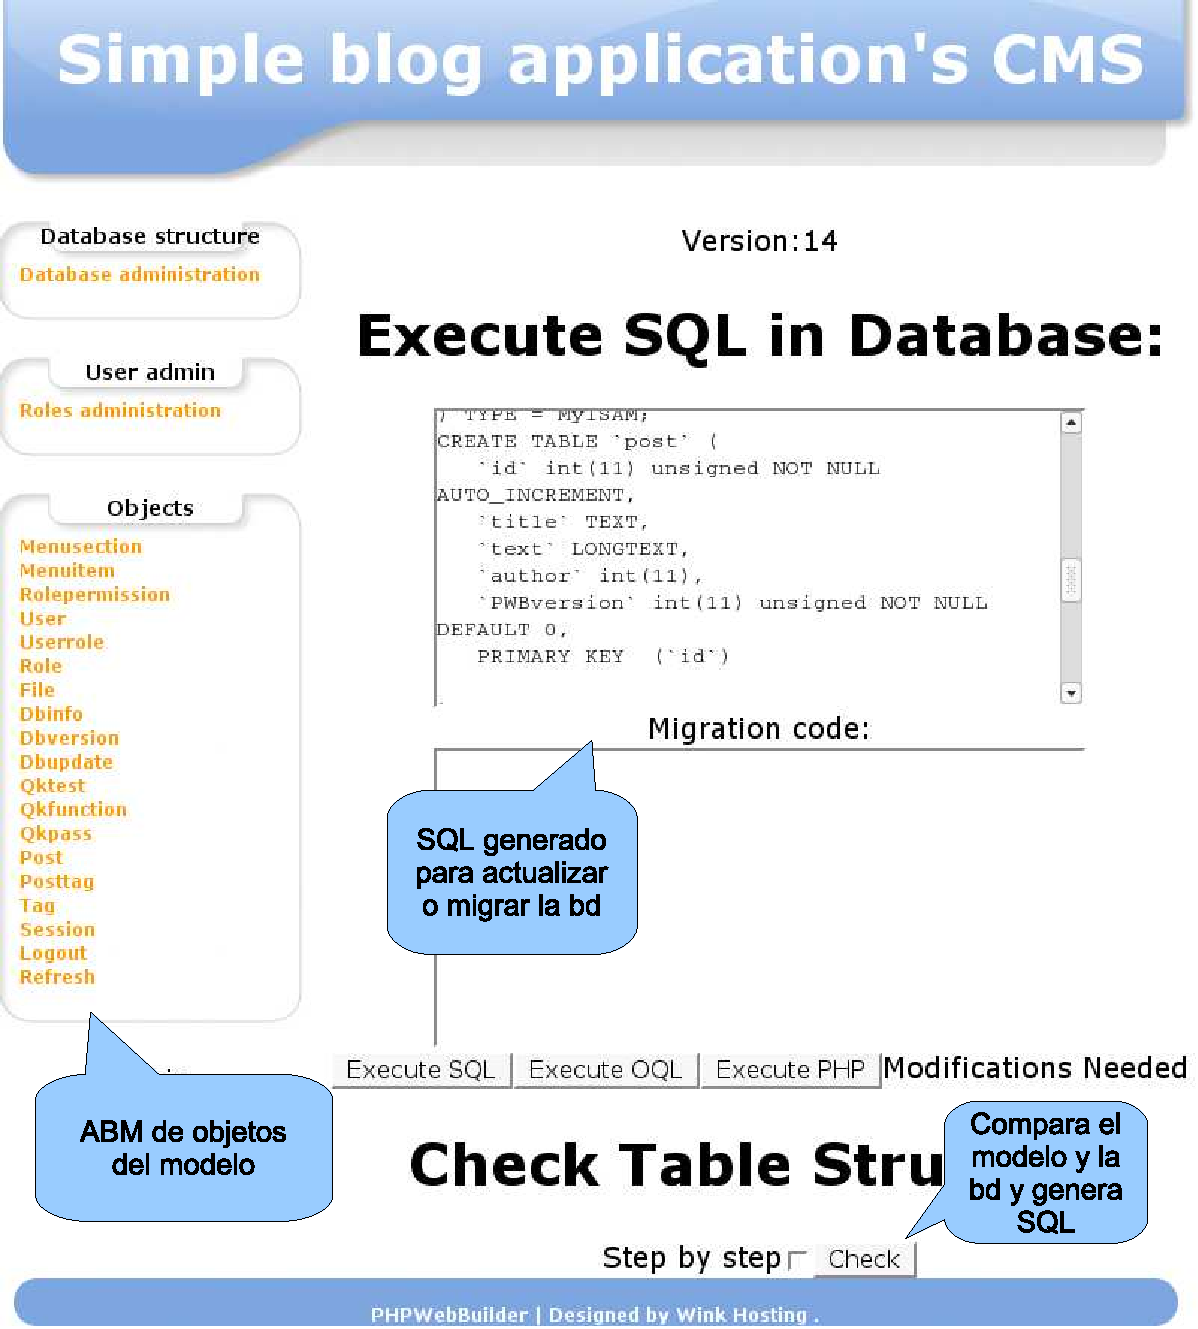
\includegraphics[scale=0.8]{images/admin2.eps}
	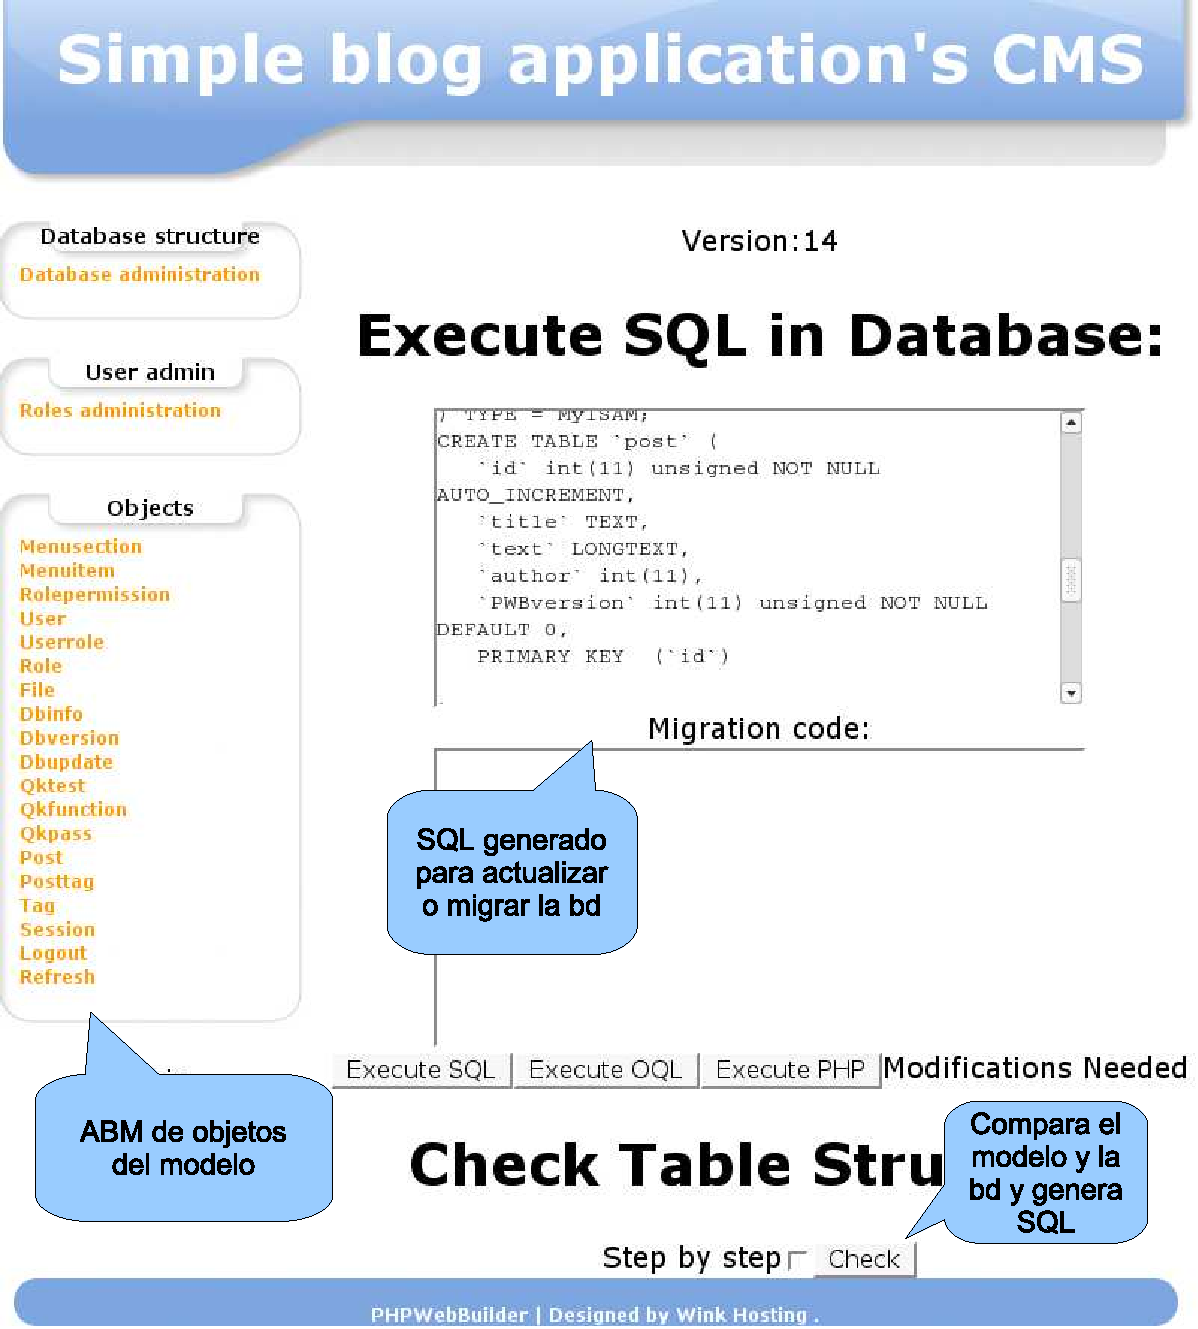
\includegraphics[scale=0.5]{images/admin2.pdf}
 	\caption{Adaptación de base de datos}
 	\label{fig-admin1}
\end{figure}

Además, podemos verificar que el esquema de base de datos sea el correcto, y mostrar y ejecutar las correcciones necesarias. Esto también es muy útil cuando se hace una modificación en el modelo de una aplicación y se necesita adaptar la base de datos a los nuevos cambios.

Por último, \PWB \ incluye una aplicación para la administración de los objetos del modelo como se ve en las figuras \ref{fig-abm1} y \ref{fig-abm2}.

\begin{figure}[h]
	\centering
	%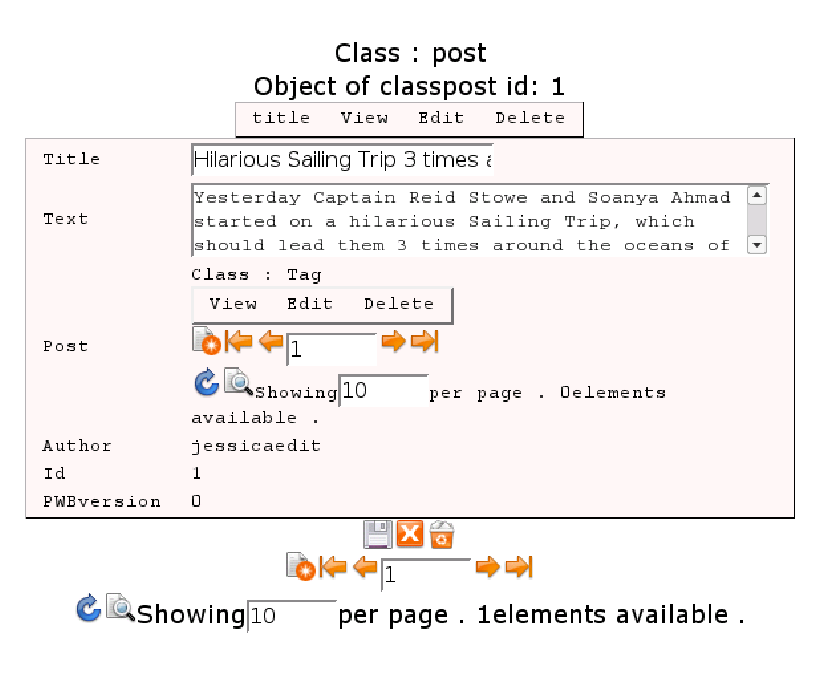
\includegraphics{images/abm1.eps}
	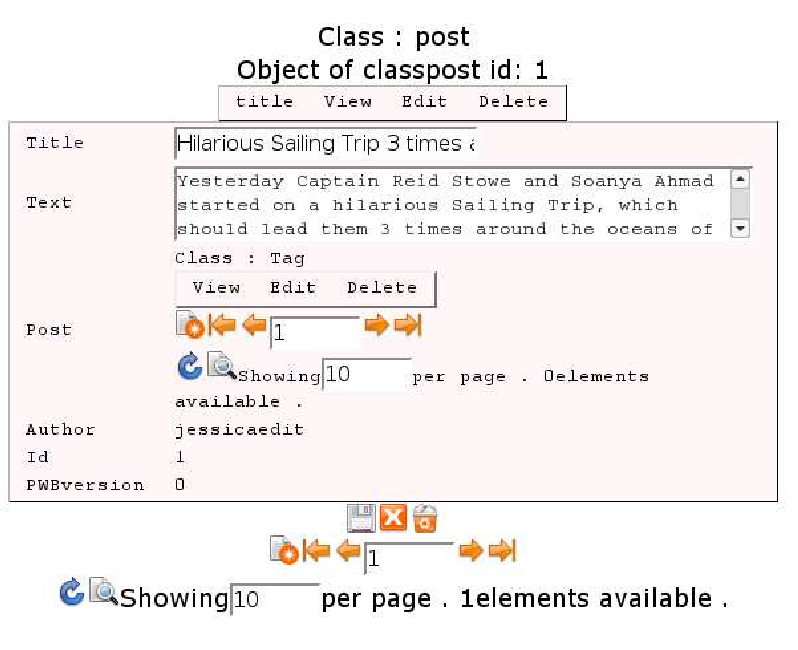
\includegraphics[scale=0.7]{images/abm1.pdf}
 	\caption{ABM Autogenerado de un Post}
 	\label{fig-abm1}
\end{figure}

\begin{figure}[h]
	\centering
	%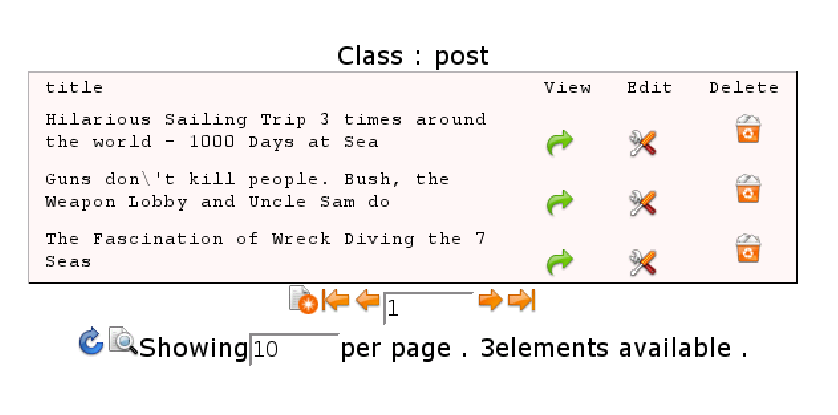
\includegraphics{images/abm2.eps}
	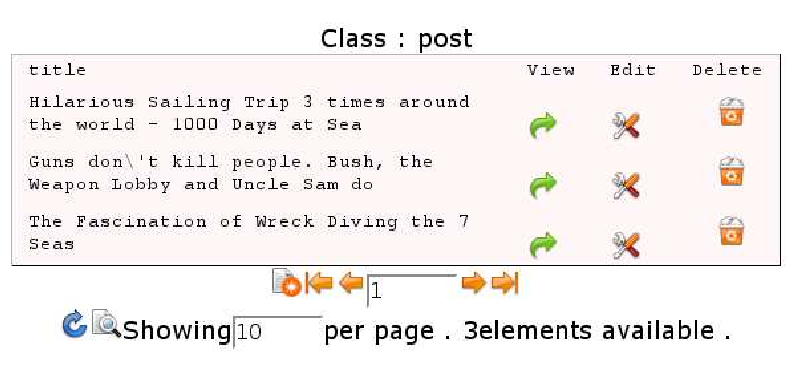
\includegraphics[scale=0.7]{images/abm2.pdf}
 	\caption{Aplicación de administración de Posts generada}
 	\label{fig-abm2}
\end{figure}

%Esta funcionalidad es provista por una herramienta que veremos más adelante.

\section{Características del Controller}
\label{sec-controller}

Teniendo ya el modelo programado y persistido, es posible implementar la interacción con el usuario. Veremos cómo listar los Posts del blog y cómo permitirle al usuario ver solamente los posts que tengan un tag.

\subsection{Componentes}
\label{sub-comp}

Las aplicaciones en \PWB\ se construyen mediante el ensamblado de componentes. Estos componentes son reutilizables ya que pueden ser parametrizados, pueden disparar eventos y pueden contener otros componentes.

El componente principal de la aplicación del blog consiste simplemente de una lista de posts. Llamemos a este componente \verb"BlogComponent".

\sourcecode{src/BlogComponent.class.php.tex}

Un componente agrega sub-componentes definiendo un método \verb"initialize" e invocando a \verb"addComponent", dejándolo como \emph{hijo} suyo en el árbol de componentes de la aplicación. Lo interesante de esta forma de diseñar la aplicación es que podemos obtener un componente a partir de otros componentes ya implementados y probados.

%Además, cada componente posee su propio flujo de control. Esto significa que podemos componer libremente, casi sin restricciones y sin preocuparnos por formularios o pasaje de parámetros por URL, conceptos que surgen al desarrollar aplicaciones web en cualquier otro framework. Por último, cada componente maneja su propia entrada de datos y actualización de vistas.

Ahora definamos la lista de \verb"Posts". Sólo basta subclasificar de \verb"CollectionNavigator", un componente general para navegación y mostrado de listados de objetos:

\sourcecode{src/PostList1.class.php.tex}

Un componente \verb"CollectionNavigator" presenta links para la navegación de los elementos (mostrándolos paginados). Para determinar cómo se van a manejar cada uno de los elementos se retorna un componente en el método \verb"addLine", en este caso un \verb'PostItem'.

Una de las ventajas que tiene esta implementación del controller es que podemos ensamblar componentes libremente, casi sin restricciones y sin preocuparnos por formularios o pasaje de parámetros por URL, conceptos que surgen al desarrollar aplicaciones web en casi cualquier otro framework.

\subsection{Widgets}
\label{sub-widget}

Necesitamos crear ahora el componente \verb'PostItem', que muestra cada \verb'Post'. Este debe mostrar el título, el texto y las etiquetas.

La interacción del usuario con la aplicación se logra por medio de \verb"Widgets"\cite{WDGTS}. Estos son componentes especiales entre los que se encuentran el componente \verb"Input", que permite recibir un string del usuario, el \verb"Text", que le presenta un texto y el \verb"CheckBox", que presenta un checkbox. Utilizaremos estos componentes para mostrar y lograr la interacción del usuario con un \verb'Post':

\sourcecode{src/PostItem1.class.php.tex}

\subsection{Control de flujo modal}
\label{sub-modal-flow}
Queremos ahora poder ver la lista de \verb"Posts" filtrada por los que tienen una determinada etiqueta al hacer click sobre ésta. Reveamos entonces nuestras clases \verb"PostItem" y \verb"PostList" para establecer la interacción necesaria.

%Veamos ahora otra característica del control de flujo de los componentes. Como vimos antes (sección \ref{sub-comp}), cada componente posee su propio flujo de control, lo que nos permitía ensamblar componentes más complejos libremente. Además de esto, la navegación a través de la aplicación se define mediante una interacción modal entre los componentes. Será mejor ver como funciona ésto en la aplicación que estamos desarrollando.

Modificamos primero la clase \verb"PostItem" para convertir las etiquetas mostradas a links. Para esto agregamos widgets de clase \verb"CommandLink" en lugar de los de clase \verb"Text" anteriores. Queremos actuar cuando una etiqueta es seleccionada, por lo tanto enviamos al padre del \verb'PostItem' que invoque el método \verb'showTag'.

\sourcecode{src/PostItem2.class.php.tex}

El \verb"CommandLink" es un \verb"Widget" especial que permite al usuario ejecutar una acción en la aplicación.

Necesitamos que la lista de \verb"Posts" se entere de que una etiqueta fue seleccionada y actuar en consecuencia. Modificamos la clase \verb"PostList" para que, al recibir el mensaje \verb'showTag' que le manda el \verb'PostItem', delegue su comportamiento a otra lista cuyos \verb"Posts" son sólo aquellos que poseen la etiqueta seleccionada. La delegación de control se logra mediante la invocación del método \verb"call". Desde el punto de vista de la vista, la delegación de control implica que el componente llamante reemplazará su vista por la del componente llamado.

\sourcecode{src/PostList2.class.php.tex}

Sería bueno que una vez mostrada la lista de posts con una determinada etiqueta podamos volver a la lista de posts de la que partimos (figura \ref{fig-blog2}). Para esto utilizamos un botón \verb"volver" cuyo comportamiento será hacer \verb"callback" sobre la nueva lista como mostramos a continuación:

\sourcecode{src/PostList3.class.php.tex}

Como se puede ver, se pueden agregar componentes fuera del método initialize, en este caso en el \verb'addBackButton'. Cuando un componente es modificado de manera dinámica, solamente sus cambios se actualizan en la vista (por ejemplo, mediante AJAX - sección \ref{sub-render}).

\begin{figure}[h]
	\centering
	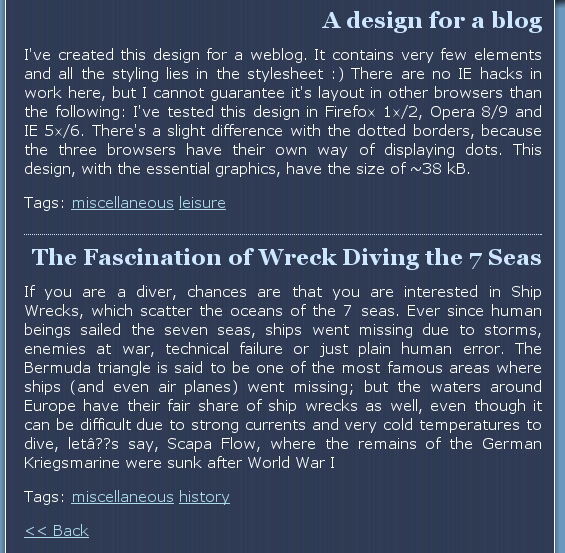
\includegraphics[scale=0.7]{images/blog2.png}
 	\caption{Posts con etiqueta 'miscellaneous' y el botón para volver}
 	\label{fig-blog2}
\end{figure}

La interacción es modal ya que el componente que llama a otro mediante \verb"call", le cede el control, que pasa al componente llamado hasta que haga \verb'callback'. Una vez hecho el \verb'callback' el control vuelve al componente llamante para que continúe con su ejecución. A nivel de vista, la vista del componente llamante es reemplazada por la del componente llamado. Esta forma de interacción es similar al uso de diálogos en aplicaciones de tipo desktop. En éstas, abrir un diálogo de forma modal bloquea el acceso a toda la aplicación. Nuestra forma de interacción modal sólo bloquea al componente llamante y por lo tanto sólo a una parte específica de la aplicación. Esa es la principal diferencia con respecto a la utilización de diálogos modales en aplicaciones de tipo desktop tradicionales.

\subsection{Multiple Dispatching y Context Dispatching}
\label{sub-dispatch}

Otra característica llamativa, es el múltiple dispatching de funciones.
Dado que muchas veces el método a utilizar depende de más de una clase, las funciones de múltiple dispatching nos ayudan a resolver este problema.

Primero se define la función, con los parametros a utilizar tipados, y luego se hace el llamado, que utiliza los tipos de los parámetros para resolver el método a utilizar.

Además, las funciones de múltiple dispatching pueden ser utilizadas pasando el contexto (la rama de componentes dentro de la que se hace el llamado) de aplicación, para de esta manera poder responder de manera diferente a un evento, dependiendo del contexto.


Por ejemplo (saliendo del ejemplo del blog), podemos tener un componente TaskList que muestre las tareas realizada en un día. Para cada tarea muestra la descripción, la hora, y el nombre de quién la completó en un componente TaskList. Si luego quisiéramos ver las tareas realizadas por uno de los usuarios, nos interesaría ver la hora, la descripción, pero no el nombre del usuario, porque ya se sabe por el contexto. Podríamos usar en ese caso un componente UserTaskShow.

Para implementar esa diferencia, una forma común sería tener 2 componentes, TaskList y UserTaskList. Esto duplica código, y además es difícil de implementar cuando el contexto de los componentes es de varios componentes (ya que tendríamos que hacer un nuevo componente para cada elemento en la rama de componentes hasta llegar al que realmente implementa la diferencia).

Entonces, podemos utilizar el Context Dispatching para elegir un componente UserTaskShow, en lugar del otro, el TaskShow, independientemente del nivel de anidamiento del componente que hace el dispatch y el componente que provee el contexto.

\section{Características de la Vista}

Con la interacción de la aplicación ya implementada, falta presentar la información al usuario de manera entendible.

\label{sec-view}
\subsection{Templates}
\label{sub-templates}

Necesitamos darle formato a los datos a presentarle al usuario. Para ésto utilizaremos templates, que se adaptan a cada uno de los componentes.

Para el \verb'PostItem', mostramos de manera resaltada el título, y el cuerpo, y más abajo los tags:

\begin{verbatim}

<templates>
  <template class="PostItem">
    <h1 id="titulo" />
    <p id="texto" />
    Tags: <div id="tags"><container class="CommandLink"/> </div>
    <hr/>
  </template>
</templates>

\end{verbatim}

Hacemos un template para los componentes de clase \verb'PostItem', asociamos al subcomponente de id \emph{titulo} al elemento \verb'h1' del html, el de id \emph{texto} al \verb'p'. Por último, hacemos un \verb'div' para el componente de id \emph{tags}, y decimos que posicione a los \verb'CommandLink' hijos de \emph{tags} con su template default.

Los templates tienen las siguientes características:
\begin{itemize}
\item Los templates se ``heredan'', así que un Componente subclase de otro que tiene template, hereda de este el template (siempre y cuando no tenga uno más específico).
También son heredables por \verb"Mixins" (sección \ref{sub-mixins}).

\item Los templates son declarativos: No incluyen comandos ni iteradores (como tienen otros engines de templates). De esta manera, el control de la aplicación está 100\% en los componentes, y además nos aseguramos que los templates generen un XML bien formado.

\item Los templates están basados en XML, con un par de tags extras (\verb"<template>" y \verb"<container>"), así que se puede generar cualquier XML (como XHTML) para mostrar los componentes.
\end{itemize}

Además, cada componente tiene un template default, por lo que no se necesita crearle uno para tener la aplicación funcionando (en nuestro caso, no lo hicimos para el \verb'CommandLink', el \verb"BlogComponent" ni el \verb"PostList").

\subsubsection{Adaptación de Diseños existentes}
\label{sub-templates-adapt}
Debido a que los templates son XML, se puede tomar una página en HTML y agregarle los tags \verb"<template>" y \verb"<container>" donde se quiera, y de esta manera conseguir un template a muy bajo costo. Además, como los templates se heredan, utilizando
\verb"Mixins" (sección \ref{sub-mixins}) y
subclases, una aplicación puede tener un diseño completo en sólo 3 o 4 templates.

\subsection{Renderings}
\label{sub-render}

Una técnica muy utilizada en las aplicaciones web 2.0, es el rendereo de cambios mediante AJAX, que permite al usuario ejecutar varias tareas en simultáneo en la aplicación y refrescar la pantalla sin recargar todo.

El rendereo (generación de la interfaz) de la aplicación se hace 100\% mediante \PWB, de modo que no hay intervención por el programador.

La manera de cambiar el engine de rendereo es tan simple como cambiar en el archivo de configuración, donde dice \verb"page_renderer=StandardPageRenderer" por \verb"page_renderer=AjaxPageRenderer", o incluso por \verb"page_renderer=CometPageRenderer" o \verb"page_renderer=XULPageRenderer".

\subsubsection{AJAX y Comet}

Todo lo generado por \PWB \ es XML bien formado, de modo que de manera transparente podemos renderear en AJAX.

Comet es una tecnología similar a AJAX que se caracteriza por mantener una conexión abierta entre el browser y el servidor en todo momento. \PWB \ aprovecha esto, ya que un importante tiempo de procesamiento de los scripts PHP es la carga del script y los datos de la sesión de usuario, que en este caso quedan vivos en la memoria del servidor.

Mediante pasaje de mensajes de otro script que envía los datos a la aplicación \PWB \ ejecutándose, podemos mantener la sesión en memoria, mejorando los tiempos de respuesta e incluso modificando la aplicación del usuario. Esta modificación puede surgir a partir de la generación de un evento por parte del usuario (por ejemplo, un click del mouse) o por sucesos ajenos a ésto, como puede ser la modificación de base de datos.

\subsubsection{XUL}

El proyecto Mozilla incluye un subproyecto llamado XUL\cite{XUL}. XUL es un lenguaje de definición de interfaces desktop en XML. Dado que la salida de la aplicación debe ser un XML bien formado y que la interacción usuario-interfaz se hace mediante javascript, \PWB \ soporta un XUL Page Renderer que renderea aplicaciones en XUL. La diferencia para el programador se encuentra en el trato de las etiquetas de los templates ya que debe utilizar elementos XUL en lugar de HTML.

Dado que los templates de HTML llevan extensión .xml y los de xul .xul, la misma aplicación, con tener templates de los 2 tipos para cada componente, puede ser rendereada de las 2 maneras.

\section{Características de \PITS}

% Si queremos poner lo siguiente, nombrar las herramientas:
%La complejidad de una aplicación por lo general es mayor que en el ejemplo anterior. \PWB\ posee otras herramientas que ayudan en la generación de los componentes y del modelo.

\subsection{BugNotifier}

\PWB \ incluye un \verb"BugNotifier", que automatiza el manejo de errores ``no manejados'' , permitiendo al usuario que encuentra una condición de error dentro de la aplicación, enviar el reporte de error a un mail configurado a tal fin, y también reiniciar la aplicación para continuar utilizándola.

En caso de que en la aplicación de Blog se encuentre un error, en lugar de presentarle al error, se le presentará con un dialogo.

\subsection{Eventos}
\label{sub-events}

En nuestra implementación, el \verb"PostItem" tiene un \verb"CommandLink" que le envía a su componente padre el mensaje \verb"showTag" cuando un tag es seleccionado. Esto trae problemas de composicionalidad, ya que no podríamos usarlo como hijo de un componente que no entienda el mensaje \verb"showTag" (ver figura \ref{fig-comp1}).

\begin{figure}[h]
	\centering
	\includegraphics*[scale=0.30]{images/componentes.png}
 	\caption{Componentes que no utilizan Eventos}
 	\label{fig-comp1}
\end{figure}

Para realmente mantener la composicionalidad, necesitamos que el \verb"PostItem" no envíe un mensaje al componente padre, pero al mismo tiempo, desde el \verb'PostList' necesitamos saber que se hizo click en el tag. Para esto, utilizamos eventos. El componente \verb'PostItem' dispara un evento cuando se hace click en un tag, y el \verb'PostList', que escucha cuando este evento se dispara, actualiza la lista de posts.

\PWB\ implementa un mecanismo simple de eventos. Todo objeto \verb"PWBObject" implementa los mensajes \verb"addInterestIn", que permite a otro objeto escuchar un evento, y \verb"triggerEvent", que dispara un evento.

Utilizando eventos, implementamos:

\sourcecode{src/PostListEvents.class.php.tex}

Al crear el \verb'PostItem', el \verb'PostList' se queda escuchando el evento \verb'tag_selected' de él, y que cuando ocurra, se le envíe el mensaje \verb'showTag'.

\sourcecode{src/PostItemEvents.class.php.tex}

El \verb'PostItem', en lugar de mandar un mensaje a su padre, se envía a sí mismo el mensaje \verb'tagSelected', que dispara un evento \verb'tag_selected', sin preocuparse de quién esté escuchando.

Existen objetos que disparan algunos eventos por default:
\begin{itemize}
\item Los \verb"Widgets", en cada acción del usuario (cuando hace click, cuando se modifica un elemento).
\item Los objetos del modelo (\verb"PersistentObject"), cuando son modificados.
\end{itemize}

Hay 2 momentos para la ejecución de respuestas a eventos: En el momento de creación del evento, o luego de la ejecución de la rama de programa, al finalizar las otras tareas. En este último caso, es posible ejecutar una sola o una vez por cada disparo del mismo evento. Esto se especifica en el \verb'addInterestIn'.

\subsection{Weak References} \label{sub-weak}
Cuando un objeto \verb"$x" queda escuchando un evento de un \verb"PWBObject" \verb"$y", este último necesita guardar una referencia al primero. En caso de que, por el flujo de la aplicación, \verb'$x' deje de ser necesario, el mecanismo de garbage collection de PHP no puede descartarlo, porque \verb'$y' lo conserva referenciado, aunque no lo necesite realmente.

Por esto implementamos un mecanismo de Weak References, en donde \verb"$y" se queda con una referencia de \verb"$x", pero de la cual el garbage collector no se entera, permitiendo borrar a \verb"$x" en caso de que sea necesario.
%$

\subsection{PHPCC}
\label{sub-phpcc}
Para crear el lenguaje OQL, debimos crear un Compiler Compiler para PHP (otros conocidos son Bison\cite{BISON}, yacc\cite{YACC}).
De esta manera ahora también se puede extender el framework con múltiples DSLs (Domain-Specific Languages - Lenguages específicos de Dominio).

\subsection{Macros}
\label{sub-macros}

Un tiempo grande del desarrollo se destina a la corrección de errores. Una modificación de un módulo de programa puede afectar a otros módulos que lo utilicen, provocando un error difícil de detectar, y por ende costoso de solucionar. Una forma de detectar estos errores es mediante el chequeo de tipos y las aserciones, que permiten un control más estricto sobre los datos que se comunican entre módulos.

La ejecución de estas validaciones, si bien son útiles para el desarrollo, consumen un tiempo innecesario cuando el programa es instalado en producción. Una forma de recortar estos tiempos es eliminar del código final todos los chequeos, pero muchos pueden pasar sin ser detectados y pueden llegar a ser útiles ante una modificación posterior del sistema.

Por esto mismo, en \PWB\ utilizamos \verb'#@typecheck@#' y \verb'#@check@#' para insertar validaciones desactivables en el código.

Por ejemplo, escribiendo \verb"#@typecheck $post: Post@#" se chequea que la variable \verb"$post"
sea un \verb'Post'. En las opciones de configuración de la aplicación, habilitamos o deshabilitamos el typechecking y el chequeo no se incluye.

\sourcecode{src/PostItemCheck.class.php.tex}

Esto avisará al programador por problemas durante el desarrollo al intentar inicializar erróneamente un \verb"PostItem" con algo que no sea un \verb'Post'.

Habilitando o deshabilitando en el config.php (sección \ref{sub-config}) \verb'compile=typecheck', podemos utilizar estos chequeos.

Tanto el OQL (sección \ref{sub-oql}) como \verb'check' y \verb'typecheck' son macros: fragmentos de código que se ejecutan una sola vez, en tiempo de compilación, y reemplazan su texto en el código de la aplicación final.

Un programador puede agregar sus propias macros declarando una función simple de PHP \verb"mi_macro" y luego llamándola con \verb"#@mi_macro" {\it parámetros} \verb"@#". Como se ve en lenguajes como C, las macros pueden llegar a tener un rol muy importante en un proyecto ya que son otra forma de modularización.
\subsection{Mixins}
\label{sub-mixins}

%Post, Tag, User
%Componentes: PostItem, PostList, BlogComponent.

Otra funcionalidad interesante es una implementación limitada de \verb"Mixins" (mediante \verb"Macros").

Un \verb"Mixin" es una forma de agrupar funcionalidad y agregársela a múltiples clases de objetos sin que estas clases estén conectadas por subclasificación. Es lo que vemos como el mejor trade-off entre simple y múltiple herencia.

\begin{verbatim}
#@mixin ValueHolder {
  var $value;
  function getValue(){
    return $this->value;
  }
  function setValue($value){
    $this->value = $value;
  }
}@#

class Contador{
  #@use_mixin ValueHolder@#
  function increment(){
    $this->setValue($this->getValue()+1);
  }
}

class Direccion extends PersistentObject{
  #@use_mixin ValueHolder@#
  function initialize(){
    $this->addField(new TextField(array('fieldName'=>'value')));
  }
}

\end{verbatim}

De esta manera podemos implementar una sola vez el comportamiento de \verb'ValueHolder' y utilizarlo en 2 clases distintas (\verb"Direccion" y \verb"Contador"), sin necesidad de relacionarlos por herencia.

Además, agregamos a los mixins en el chequeo de tipos. Si tenemos un \\ chequeo \verb"#@typecheck $v: ValueHolder@#", tanto un objeto de clase \verb"Direccion" como uno de clase \verb"Contador" cumplen con la condición.

\subsection{Múltiples Configuraciones}
\label{sub-config}
Para el desarrollo colaborativo, es útil mantener múltiples configuraciones. O para trabajar en distintos clientes. O para hacer testing y deployment.

Por todo esto, \PWB \ mantiene un archivo de configuraciones múltiples para adaptar cada una a una necesidad específica. En un archivo de configuración global (config.php) se guardan las variables específicas de cada configuración, además de las variables comunes a todas. Luego, en otro archivo (serverconfig) se pone la configuración que se va a utilizar.

\subsection{Compilación}

El uso de macros y la inclusión de los muchos archivos de \PWB, hacen que la carga en cada request pueda ser muy lenta. Por eso implementamos una mini-compilación de los archivos PHP (para que las macros ya estén procesadas) y además habilitamos varios outputs de esta compilación del código (todo a un sólo archivo PHP, sólo las clases utilizadas a un archivo PHP, en archivos separados). Esta configuración es seteable desde los archivos de configuración.

%\section{Trabajos Hechos}
%Entre los trabajos que hicimos, se encuentran sitios web y sistemas de intranet.

\section{Related Work}

Gran parte de nuestra inspiración del ``Controller'' vino de SeaSide \cite{seaside}, un Framework de AppsWeb en Smalltalk.

Las ideas de los Componentes, eventos, weakreferences y callbacks entre Componentes, fueron tomadas de Seaside.

Dejamos de lado el Smalltalk, usando PHP, y el ``HTML Programático'', en lugar de los cuales utlizamos nuestros ``Templates Declarativos'' .

Smalltalk tiene Traits \cite{traits}, de los que nosotros inspiramos nuestros Mixins. En realidad, los mixins son conceptos anteriores, similares a nuestros mixins. Los Traits no tanto.
\begin{verbatim}
Widgets http://en.wikipedia.org/wiki/GUI_Widget

El proyexto XUL www.mozilla.org/projects/xul/. Los renderers transparentes.

Yacc dinosaur.compilertools.net/yacc/index.html, Bison www.gnu.org/software/bison/ y Parsec www.cs.uu.nl/~daan/parsec.html.
OQL http://www.odmg.org/. DSLs http://homepages.cwi.nl/~arie/papers/dslbib/.

Persistencia: Hibernate www.hibernate.org/, Por alcance: JDO www.jpox.org/.

Macros. http://en.wikipedia.org/wiki/C_preprocessor

Compilación. http://www.phpclasses.org/browse/package/3215.html

Zope, http://www.symfony-project.com/,

http://www.phpmvc.net/,

http://www.cakephp.org/,

http://seagull.phpkitchen.com/,

http://www.struts4php.org/,

http://www.mojavelinux.com/projects/studs/.

http://dev.helma.org/
\end{verbatim}



\section{Conclusiones}

\PWB\ no presenta en sí conceptos novedosos, sino que reúne las opciones que consideramos mejores, y los integra e interrelaciona dentro del mismo framework. Esto libera a los desarrolladores de muchas decisiones reiterativas, y les permite enfocarse en los problemas específicos de la aplicación a desarrollar.

Los próximos pasos a realizar son: implementar mejoras en el manejo de colecciones en el modelo, e implementar persistencia por alcance \cite{jpox,jdo}.

%Aún quedan cosas por hacer. Algunas de ellas son implementar mejoras en el manejo de colecciones en el modelo, documentar, agregar soporte DSLs composicionales, mejorar la integración y comunicación de múltiples aplicaciones y diseñar e implementar templates paramétricos y dependientes del contexto y implementar persistencia por alcance similar a JDO \cite{jpox}.


%\section{Agradecimientos}

\newpage
\bibliography{references}
\bibliographystyle{plain}

\setcounter{section}{0}
\newpage
\section*{Apéndices}
\section{Código completo}

\begin{lgrind}
% Remember to use the lgrind style

\Head{}
\File{src/Post.class.php}{2007}{4}{24}{22:26}{509}
\L{\LB{\<?\V{php}}}
\L{\LB{}}
\L{\LB{\K{class}_\V{Post}_\K{extends}_\V{PersistentObject}_\{}}
\index{initialize}\Proc{initialize}\L{\LB{}\Tab{2}{\K{function}_\V{initialize}()_\{}}
\L{\LB{}\Tab{4}{\N{\$this}\-\!\>\V{addField}(\K{new}_\V{TextField}(\K{array}(\S{}{'}fieldName{'}\SE{}=\>\S{}{'}title{'}\SE{})));}}
\L{\LB{}\Tab{4}{\N{\$this}\-\!\>\V{addField}(\K{new}_\V{TextArea}(\K{array}(\S{}{'}fieldName{'}\SE{}=\>\S{}{'}text{'}\SE{})));}}
\L{\LB{}\Tab{4}{\N{\$this}\-\!\>\V{addField}(\K{new}_\V{CollectionField}(}}
\L{\LB{}\Tab{6}{\K{array}(}}
\L{\LB{}\Tab{8}{\S{}{'}fieldName{'}\SE{}=\>\S{}{'}tags{'}\SE{},}}
\L{\LB{}\Tab{8}{\S{}{'}direct{'}\SE{}=\>\K{false},}}
\L{\LB{}\Tab{8}{\S{}{'}JoinType{'}\SE{}=\>\V{PostTag},}}
\L{\LB{}\Tab{8}{\S{}{'}targetField{'}\SE{}=\>\S{}{'}tag{'}\SE{},}}
\L{\LB{}\Tab{8}{\S{}{'}reverseField{'}\SE{}=\>\S{}{'}post{'}\SE{})}}
\L{\LB{}\Tab{7}{)}}
\L{\LB{}\Tab{4}{);}}
\L{\LB{}\Tab{4}{\N{\$this}\-\!\>\V{addField}(\K{new}_\V{IndexField}(\K{array}(\S{}{'}fieldName{'}\SE{}_=\>_\S{}{'}author{'}\SE{},_\S{}{'}type{'}\SE{}_=\>_\S{}{'}User{'}\SE{})));}}
\L{\LB{}\Tab{2}{\}}}
\L{\LB{\}}}
\L{\LB{?\>}}

\end{lgrind}

\begin{lgrind}
% Remember to use the lgrind style

\Head{}
\File{stdin}{2007}{4}{29}{10:35}{0}
\L{\LB{\K{class}_\V{Tag}_\K{extends}_\V{PersistentObject}_\{}}
\index{initialize}\Proc{initialize}\L{\LB{}\Tab{8}{\K{function}_\V{initialize}()_\{}}
\L{\LB{}\Tab{16}{\N{\$this}\-\!\>\V{addField}(\K{new}_\V{TextField}(\K{array}_(}}
\L{\LB{}\Tab{24}{\S{}{'}fieldName{'}\SE{}_=\>_\S{}{'}nombre{'}\SE{},}}
\L{\LB{}\Tab{24}{\S{}{'}is\_index{'}\SE{}_=\>_\K{true}}}
\L{\LB{}\Tab{16}{)));}}
\L{\LB{}\Tab{16}{\N{\$this}\-\!\>\V{addField}(\K{new}_\V{CollectionField}(\K{array}_(}}
\L{\LB{}\Tab{24}{\S{}{'}fieldName{'}\SE{}_=\>_\S{}{'}posts{'}\SE{},}}
\L{\LB{}\Tab{24}{\S{}{'}direct{'}\SE{}_=\>_\K{false},}}
\L{\LB{}\Tab{24}{\S{}{'}JoinType{'}\SE{}_=\>_\S{}{'}PostTag{'}\SE{},}}
\L{\LB{}\Tab{24}{\S{}{'}targetField{'}\SE{}_=\>_\S{}{'}post{'}\SE{},}}
\L{\LB{}\Tab{24}{\S{}{'}reverseField{'}\SE{}_=\>_\S{}{'}tag{'}\SE{}}}
\L{\LB{}\Tab{16}{)));}}
\L{\LB{}\Tab{8}{\}}}
\L{\LB{\}}}
\L{\LB{}}
\L{\LB{\K{class}_\V{PostTag}_\K{extends}_\V{PersistentObject}_\{}}
\index{initialize}\Proc{initialize}\L{\LB{}\Tab{8}{\K{function}_\V{initialize}()_\{}}
\L{\LB{}\Tab{16}{\N{\$this}\-\!\>\V{addField}(\K{new}_\V{IndexField}(\K{array}_(}}
\L{\LB{}\Tab{24}{\S{}{'}fieldName{'}\SE{}_=\>_\S{}{'}post{'}\SE{},}}
\L{\LB{}\Tab{24}{\S{}{'}type{'}\SE{}_=\>_\V{Post},}}
\L{\LB{}\Tab{24}{\S{}{'}is\_index{'}\SE{}_=\>_\K{true}}}
\L{\LB{}\Tab{16}{)));}}
\L{\LB{}\Tab{16}{\N{\$this}\-\!\>\V{addField}(\K{new}_\V{IndexField}(\K{array}_(}}
\L{\LB{}\Tab{24}{\S{}{'}fieldName{'}\SE{}_=\>_\S{}{'}tag{'}\SE{},}}
\L{\LB{}\Tab{24}{\S{}{'}type{'}\SE{}_=\>_\V{Tag},}}
\L{\LB{}\Tab{24}{\S{}{'}is\_index{'}\SE{}_=\>_\K{true}}}
\L{\LB{}\Tab{16}{)));}}
\L{\LB{}\Tab{8}{\}}}
\L{\LB{\}}}

\end{lgrind}

\end{document}